%----------------------------------------------STANDARDIZATION------------------------------------------------
\documentclass[conference]{IEEEtran}

\usepackage{cite}
\usepackage{amsmath,amssymb,amsfonts}
\usepackage{algorithmic}
\usepackage{graphicx}
\usepackage{textcomp}
\usepackage{xcolor}
\usepackage{url}
\usepackage{float}
\usepackage{gensymb}

% Remove unnecessary packages and formatting
% ...existing code until \begin{document}...

\begin{document}

\title{PID Controller Implementation in CARLA Simulator}

\author{
    \IEEEauthorblockN{Andre T S Hucke\textsuperscript{1}, Samir A Gupta\textsuperscript{2}, Dubey Abhishek\textsuperscript{2}}
    \IEEEauthorblockA{\textsuperscript{1}Department of Electrical and Computer Engineering, Vanderbilt University, Tennessee, USA}
    \IEEEauthorblockA{\textsuperscript{2}Department of Computer Science, Vanderbilt University, Tennessee, USA}
}

\maketitle

\section{Introduction}

The pursuit of fully autonomous vehicles has accelerated in recent years, driven by advancements in artificial intelligence, machine learning, and sensor technologies. However, the complexities and safety concerns associated with real-world testing have led to an increased reliance on simulation environments. CARLA \cite{dosovitskiy2017carla}, an open-source simulator developed by the Computer Vision Center at the Universitat Autònoma de Barcelona, provides a flexible and powerful platform for developing and testing autonomous driving algorithms.

PID (Proportional-Integral-Derivative) controllers play a crucial role in the control systems of autonomous vehicles, particularly in managing steering and speed control. These controllers are favored for their simplicity and effectiveness in maintaining desired vehicle trajectories and velocities \cite{10.1108/ir-12-2019-0254}. Before real-world implementation, a safe simulated environment is preferred. CARLA has emerged as an excellent platform for autonomous driving simulation, allowing researchers to implement custom solutions using Python. It supports the development of autonomous vehicles by providing a realistic urban environment where various driving scenarios can be simulated.

This research aims to enable a vehicle to accurately follow a predefined route and maintain the desired speed while ensuring stability and minimizing collision risks, thereby enhancing knowledge in cyber-physical systems and PID control. The core components of this project include:

\begin{itemize}
    \item \textbf{Waypoint Planning:}
        \begin{itemize}
            \item Creating routes using camera-based waypoint generation.
            \item Processing waypoints to determine target trajectories.
        \end{itemize}

    \item \textbf{Vehicle Control:}
        \begin{itemize}
            \item Implementing PID controllers for throttle, brake, and steering.
            \item Following paths while maintaining desired speed.
        \end{itemize}

    \item \textbf{Collision Detection:}
        \begin{itemize}
            \item Integrating a collision sensor system.
        \end{itemize}

    \item \textbf{Performance Metrics:}
        \begin{itemize}
            \item Reaching the destination (end waypoint).
            \item Monitoring speed adherence.
            \item Measuring lateral error compared to the route.
            \item Analyzing time within thresholds.
        \end{itemize}
\end{itemize}

\subsection{Hypotheses}

\begin{itemize}
    \item \textbf{Hypothesis 1:} Implementing a PID controller will enable the vehicle to follow the route accurately while maintaining the target speed within acceptable thresholds.
        \begin{itemize}
            \item Fine-tuning PID parameters will minimize speed deviations and improve path tracking.
            \item \textbf{Expected outcome:} The vehicle maintains the target speed with minimal throttle and brake oscillations.
        \end{itemize}

    \item \textbf{Hypothesis 2:} A properly configured PID controller for steering will minimize lateral error and keep the vehicle close to the centerline.
        \begin{itemize}
            \item Appropriate PID term combinations will enable stable correction of lateral deviations.
            \item \textbf{Expected outcome:} Low average lateral error (less than 1 meter from the route centerline).
        \end{itemize}

    \item \textbf{Hypothesis 3:} No collisions will occur as long as the path remains within road boundaries.
        \begin{itemize}
            \item A collision sensor will detect any impacts that occur.
            \item \textbf{Expected outcome:} The vehicle stops promptly upon collision detection.
        \end{itemize}
\end{itemize}

\section{Related Work}

Previous research underscores the integral role of PID controllers in steering systems, enabling vehicles to follow desired paths by adjusting steering angles based on feedback from the vehicle's position relative to the path \cite{10.5772/51314,10.25165/j.ijabe.20241701.7296}. Studies discuss how PID controllers are employed in Lane Keeping Assistance Systems (LKAS) to ensure that vehicles remain centered in their lanes by applying corrective steering forces when deviations are detected \cite{10.4218/etrij.15.0114.0123}. Additionally, PID controllers are utilized in longitudinal velocity control to manage the speed of autonomous vehicles by adjusting throttle positions to achieve smooth acceleration and deceleration \cite{10.22214/ijraset.2021.32866}, which enhances passenger comfort and ensures safety during operation.

The adaptability of PID controllers is further emphasized in research exploring adaptive PID control systems that adjust to varying conditions, thereby improving the vehicle's response to dynamic environments \cite{10.5772/51314}. Despite the advantages of PID controllers, there are notable gaps in knowledge regarding their limitations in complex driving scenarios. While PID controllers are effective for straightforward path tracking, they may struggle with non-linear dynamics and external disturbances such as sudden obstacles or changes in road conditions \cite{10.25165/j.ijabe.20241701.7296}. This limitation necessitates further research into hybrid control strategies that integrate PID with advanced control methods like Model Predictive Control (MPC) or fuzzy logic systems to enhance robustness and adaptability in real-world applications \cite{10.2478/auseme-2020-0003,10.1088/1742-6596/2478/6/062003}.

Current literature indicates a need for more comprehensive studies on integrating PID controllers with emerging technologies such as machine learning and sensor fusion, which could significantly improve the decision-making capabilities of autonomous vehicles \cite{10.1109/tiv.2016.2578706}. Exploring these hybrid approaches could bridge the gap between the simplicity of PID controllers and the complex demands of autonomous driving in diverse environments.

\section{Methodology}

The vehicle aims to maintain a smooth path between a series of waypoints while adhering to speed constraints. To implement the PID controller, CARLA, an open-source simulator for autonomous driving research, was employed as the simulation environment. The controller integrates the CARLA simulator with custom-developed scripts for vehicle control, route management, and data acquisition. The project was structured around a sequence of tasks, each targeting different functionalities to achieve automated path-following behavior for a simulated vehicle using Python.

Town02 was selected as the environment due to its simpler layout, ideal for testing a basic PID controller. The vehicle was spawned and controlled via appropriate commands, initialized using CARLA's blueprint library. A series of waypoints were established to define the desired route.

\subsection{System Model}

The system involves controlling the position and speed of a vehicle to follow a predefined route using a PID controller. The vehicle state is updated through a feedback mechanism that utilizes velocity and positional information. The control objectives include minimizing both longitudinal (speed) and lateral (steering) errors.

\subsection{Route Management and Waypoint Planning}
The route is defined through a series of waypoints ($w_i$) extracted from an XML file or generated through camera-based waypoint tracing. The waypoints are represented as 3D positions in the form:

\begin{equation}
w_i = (x_i, y_i, z_i)
\end{equation}

To follow the path, a target waypoint is selected using a lookahead-based approach, and the vehicle moves towards this target using weighted averaging to ensure smooth path tracking:

\begin{equation}
w_{\text{target}} = \frac{1}{W} \sum_{i=1}^{n} w_i \times \text{weight}_i
\end{equation}

where $W$ is the sum of the weights used for averaging. These weights ($\text{weight}_i$) determine the influence of each waypoint on the desired direction.

\subsection{PID Control and Vehicle Dynamics}
The PID controller is used to compute control actions for throttle, brake, and steering. For each of these control signals, the PID controller calculates an output using the following formula:

\begin{equation}
u(t) = K_p e(t) + K_i \int_{0}^{t} e(\tau) d\tau + K_d \frac{de(t)}{dt}
\end{equation}

where:
\begin{itemize}
    \item $K_p, K_i, K_d$ are the proportional, integral, and derivative gains respectively.
    \item $e(t)$ is the control error, which varies depending on the control signal (e.g., velocity or steering angle).
\end{itemize}

For each PID controller instance, the error was calculated using:

\subsubsection{Proportional Term ($p$)}

\begin{equation}
p(t) = K_p \cdot e(t)
\end{equation}

\subsubsection{Integral Term ($i$)}

\begin{equation}
i(t) = K_i \sum_{j=0}^{t} e(j) \cdot \Delta t
\end{equation}

\subsubsection{Derivative Term ($d$)}

\begin{equation}
d(t) = K_d \cdot \frac{e(t) - e(t-\Delta t)}{\Delta t}
\end{equation}

The final control action ($u(t)$) is calculated as:

\begin{equation}
u(t) = p(t) + i(t) + d(t)
\end{equation}

These control actions are used in:

\subsubsection{Throttle Control}
The target speed $v_{\text{target}}$ is compared with the current speed $v_{\text{current}}$ to calculate the speed error ($e_v = v_{\text{target}} - v_{\text{current}}$). The PID control action for the throttle is computed as:

The throttle ($T$) and brake ($B$) values are determined by the speed error. If the speed error is positive, the throttle value is increased; otherwise, braking is applied:

\begin{equation}
T = \max(0, K_p \cdot e_v + K_i \cdot \int_{0}^{t} e_v d\tau + K_d \cdot \frac{de_v(t)}{dt})
\end{equation}

\begin{equation}
B = \max(0, -K_p \cdot e_v - K_i \cdot \int_{0}^{t} e_v d\tau - K_d \cdot \frac{de_v(t)}{dt})
\end{equation}

\begin{equation}
u_{\text{throttle}} = K_p e_v + K_i \int_{0}^{t} e_v(\tau) d\tau + K_d \frac{de_v(t)}{dt}
\end{equation}

% Add the initialization parameters
The PID controller for throttle response was initialized with the following parameters:

\begin{equation}
K_p = 1.0,\quad K_i = 0.1,\quad K_d = 0.0
\end{equation}

These parameters were chosen to provide a strong proportional response for immediate error correction and a small integral action to eliminate steady-state errors. The derivative term was set to zero to avoid amplifying measurement noise and because the system's dynamics did not require derivative control.

\subsubsection{Steering Control}

The steering control aims to minimize the lateral displacement from the path. The error is represented by the angle difference between the direction vector to the target waypoint and the vehicle's current heading. The steering error ($e_s$) is defined as:

\begin{equation}
e_s = \arctan \left( \frac{y_{\text{target}} - y_{\text{current}}}{x_{\text{target}} - x_{\text{current}}} \right) - \psi
\end{equation}

where $\psi$ is the vehicle's current heading angle. The PID control action for steering is:

\begin{equation}
u_{\text{steer}} = K_p e_s + K_i \int_{0}^{t} e_s(\tau) d\tau + K_d \frac{de_s(t)}{dt}
\end{equation}

The steering value ($\delta$) is determined by the steering error and clamped within the allowable range:

\begin{equation}
\delta = \text{clip}\left( K_p \cdot e_s + K_i \cdot \int_{0}^{t} e_s d\tau + K_d \cdot \frac{de_s(t)}{dt}, -1, 1 \right)
\end{equation}

The PID controller for steering response was initialized with the following parameters:

\begin{equation}
K_p = 0.5,\quad K_i = 0.0,\quad K_d = 0.1
\end{equation}

These parameters were chosen to provide a balanced response for steering control. The proportional gain ($K_p$) was set to 0.5 to ensure a moderate response to steering errors without causing excessive oscillations. The integral gain ($K_i$) was set to 0.0 to avoid accumulation of past errors, which is not critical for steering control in this context. The derivative gain ($K_d$) was set to 0.1 to provide damping and reduce overshoot, helping to smooth out the steering response.

\subsection{Collision Detection and Performance Analysis}
\subsubsection{Collision Detection}
The vehicle's collision sensor detects impacts and computes the magnitude of the impulse force:

\begin{equation}
F_{\text{collision}} = \sqrt{F_x^2 + F_y^2 + F_z^2}
\end{equation}

If $F_{\text{collision}} > F_{\text{threshold}}$, the vehicle control switches to a full brake to stop the vehicle.

\subsection{Performance Metrics}
To evaluate speed and lateral control performance, metrics such as time within the speed threshold and lateral error are computed and plotted. These metrics are used to assess the quality of the PID tuning for both velocity and path-following accuracy.

\subsubsection{Lateral Error Calculation}

The lateral error $e_{\text{lat}}$ is calculated as follows:

\begin{enumerate}
    \item \textbf{Path Vector Calculation}

    Let the consecutive waypoints be $\wp_1 = (x_1, y_1)$ and $\wp_2 = (x_2, y_2)$. The path vector $v_p$ is:
    
    \begin{equation}
    v_p = (x_2 - x_1, y_2 - y_1)
    \end{equation}
    
    The length of the path vector is:
    
    \begin{equation}
    |v_p| = \sqrt{(x_2 - x_1)^2 + (y_2 - y_1)^2}
    \end{equation}
    
    The normalized path vector is:
    
    \begin{equation}
    v_p = \left( \frac{x_2 - x_1}{|v_p|}, \frac{y_2 - y_1}{|v_p|} \right)
    \end{equation}
    
    \item \textbf{Vector from Waypoint to Vehicle}
    
    Let the current vehicle position be $p_v = (x_v, y_v)$. The vector from $\wp_1$ to the vehicle $v_{wp \to v}$ is:
    
    \begin{equation}
    v_{wp \to v} = (x_v - x_1, y_v - y_1)
    \end{equation}
    
    \item \textbf{Lateral Error Calculation}
    
    The lateral error $e_{\text{lat}}$ is computed using the cross product of the path vector and the vector from the waypoint to the vehicle:
    
    \begin{equation}
    e_{\text{lat}} = v_{p_x} \cdot v_{wp \to v_y} - v_{p_y} \cdot v_{wp \to v_x}
    \end{equation}
    
    Expanding in terms of coordinates:
    
    \begin{equation}
    e_{\text{lat}} = \frac{(x_2 - x_1)}{|v_p|} \cdot (y_v - y_1) - \frac{(y_2 - y_1)}{|v_p|} \cdot (x_v - x_1)
    \end{equation}

\end{enumerate}

\subsubsection{Velocity Over Time Calculation}

The velocity over time calculation involves analyzing the speed of the vehicle to determine how well it maintains the target speed.

\begin{enumerate}
    \item \textbf{Speed at Each Time Interval}

    Let the target speed be $v_{\text{target}}$, and let the recorded speed at different time instances be $v_1, v_2, \ldots, v_n$, measured at times $t_1, t_2, \ldots, t_n$.

    \item \textbf{Time Intervals}

    The time intervals are given by:

    \begin{equation}
    \Delta t_i = t_{i+1} - t_i \quad \text{for } i = 1, 2, \ldots, n-1
    \end{equation}

    \item \textbf{Speed Error}

    The speed error at each time instance is defined as:

    \begin{equation}
    e_i = |v_i - v_{\text{target}}|
    \end{equation}

    \item \textbf{Time Spent Within Threshold}

    Let the speed threshold be $\epsilon$. The time spent within the threshold is calculated as the sum of the time intervals where the speed error is within $\epsilon$:

    \begin{equation}
    T_{\text{in\_range}} = \sum_{\substack{i=1 \\ e_i \leq \epsilon}}^{n-1} \Delta t_i
    \end{equation}

    \item \textbf{Total Time}

    The total time $T_{\text{total}}$ is the difference between the final and initial recorded times:

    \begin{equation}
    T_{\text{total}} = t_n - t_1
    \end{equation}

    \item \textbf{Time Outside Threshold}

    The time spent outside the threshold $T_{\text{out\_range}}$ is:

    \begin{equation}
    T_{\text{out\_range}} = T_{\text{total}} - T_{\text{in\_range}}
    \end{equation}

    \item \textbf{Performance Metrics}

    The percentage of time within and outside the threshold can be computed as follows:

    \begin{equation}
    P_{\text{in\_range}} = \frac{T_{\text{in\_range}}}{T_{\text{total}}} \times 100\%
    \end{equation}

    \begin{equation}
    P_{\text{out\_range}} = \frac{T_{\text{out\_range}}}{T_{\text{total}}} \times 100\%
    \end{equation}

\end{enumerate}

\section{Experimental Plan}

Ten user-defined routes were created using CARLA's camera as a route planner with varying complexities (eg. varying numbers of turns), and all routes were successfully completed. An example of a simulation with the route can be seen in Figure~\ref{fig:route}

\begin{figure}[h]
    \centering
    \includegraphics[width=\columnwidth]{Plots/Route.png}
    \caption{Bird's eye view a simulation with the route plotted for the user to visualize where the car is going.}
    \label{fig:route}
\end{figure}

For route tracking, a lookahead of three waypoints was set after trial and error. Using a single waypoint resulted in collisions in some scenarios while analyzing the entire path at every time point without a lookahead also led to collisions. Although an unwanted state happened in these scenarios they were useful to prove Hypothesis 3, where the simulation ended and the next started as soon as the collision happened.

Due to how the lateral error was calculated, the error increases when the vehicle navigates a turn, as shown by the spikes in Figure~\ref{fig:lateral_error}. When focusing on how well the car maintained a bearing that followed the route in straight lines, it is evident that the vehicle tracks the route well without much wobble. Performance in sharp 90-degree turns indicated the need for more advanced controllers or adaptive PID tuning strategies.

\begin{figure}[h]
    \centering
    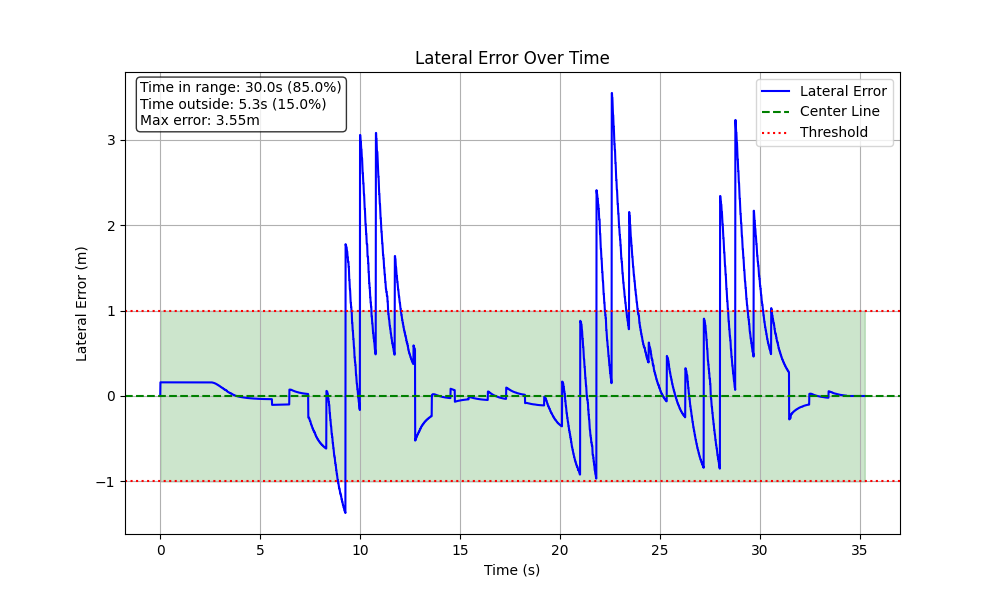
\includegraphics[width=\columnwidth]{Plots/lateral_error_waypoints0.png}
    \caption{Lateral error analysis showing the vehicle's deviation from the intended path over time. The graph demonstrates the effectiveness of the PID controller in maintaining the vehicle close to the desired trajectory.}
    \label{fig:lateral_error}
\end{figure}

Regarding speed maintenance, the PID controller was appropriately fine-tuned. Most of the time, the vehicle stayed outside the target speed during the initial acceleration period when the simulation started, and the car smoothly accelerated to reach the target speed.

\begin{figure}[h]
    \centering
    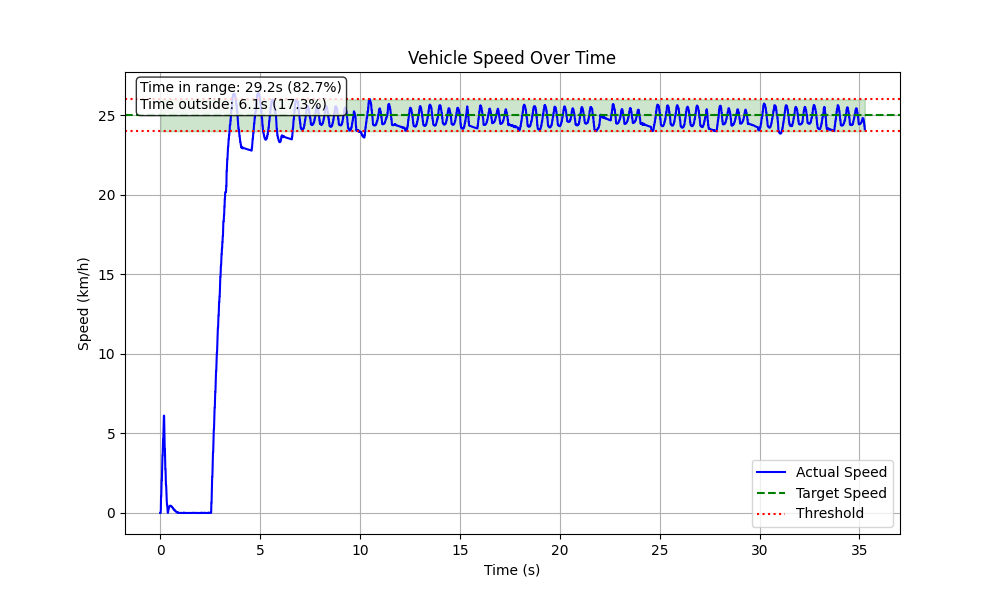
\includegraphics[width=\columnwidth]{Plots/speed_performance_waypoints0.png}
    \caption{Speed performance analysis showing the vehicle's actual speed compared to the target speed. The plot illustrates the PID controller's ability to maintain consistent speed while following the designated route.}
    \label{fig:speed_performance}
\end{figure}

Overall, the project was successful considering the defined hypotheses. The observed effect with sharp 90-degree turns was expected according to previous research \cite{10.25165/j.ijabe.20241701.7296}, but the vehicle was still able to complete all routes within the road boundaries without crashing.

\section{Conclusion}

This project successfully demonstrated the implementation of a PID controller for autonomous vehicle control within the CARLA simulator. By fine-tuning the PID parameters, the vehicle accurately followed predefined routes and maintained the target speed, thereby validating the defined hypotheses. The lateral error analysis indicated effective path tracking, particularly in straight-line segments; however, performance during sharp 90-degree turns highlighted areas for potential improvement.

Although CARLA provides advanced route planning capabilities with automatic pathfinding, this project intentionally employed more rudimentary methods. This approach facilitated a deeper understanding of the simulator and enabled exploration of how CARLA's camera features can be leveraged in future research.

Future work may involve investigating advanced control strategies or adaptive PID tuning to improve performance in complex driving scenarios. Moreover, varying the vehicle's speed, incorporating turns of various angles, experimenting with different simulation environments, and integrating computer vision techniques could facilitate the development of a fully autonomous vehicle without the need for manual route planning.

\section{Acknowledgements}

All code and additional results for other scenarios are available at \url{https://github.com/AndreHucke/CARLA_PID_PROJECT}.

ChatGPT and GitHub Copilot were used to develop and polish the code and text.

\bibliographystyle{IEEEtran}
\bibliography{References}

\end{document}
